\section{McCaskill}

McCaskill stellt eine Methode zur Berechnung der Partitionsfunktion für RNA-Sequenzen basierend auf der Boltzmann Verteilung vor, um die Strukturverteilung einer RNA-Sequenz zu berechnen.

\vspace{1.5em}

Das Problem bei Zuker ist, dass die sekundäre RNA-Struktur mit minimaler Energie nicht immer die biologisch relevanteste ist. Für sekundäre RNA-Strukturen mit geringer Energie ist es möglich, biologisch relevanter zu sein, als alle anderen möglichen sekundären RNA-Strukturen. Daher wird eine neue Möglichkeit benötigt, um diejenige RNA-Struktur heraus zu finden, die biologisch am relevantesten ist. McCaskill berechnet für eine RNA-Sequenz die Wahrscheinlichkeit der Basenpaare mit Hilfe der Boltzmann-Verteilung. Anhand der Basenpaar-Wahrscheinlichkeiten lässt sich die wahrscheinlichste sekundäre RNA-Struktur ermitteln.

\vspace{1.5em}

\tikzstyle{mybox} = [draw=blue, fill=blue!20, very thick, rectangle, rounded corners, inner sep=20pt, inner ysep=20pt, text width=0.95\textwidth]
\tikzstyle{fancytitle} =[fill=blue, text=white]
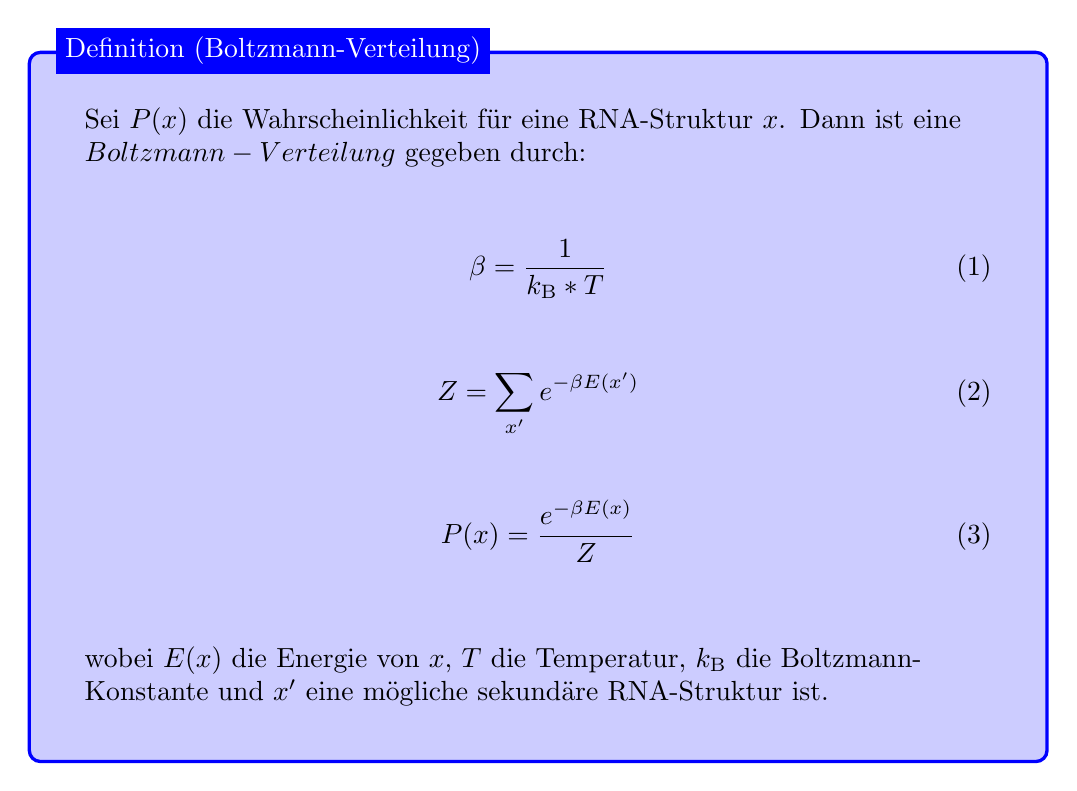
\begin{tikzpicture}
	\node [mybox] (box){%
    	Sei $P(x)$ die Wahrscheinlichkeit für eine RNA-Struktur $x$.
    	Dann ist eine $Boltzmann-Verteilung$ gegeben durch:
    	
		\vspace{1.5em}		
			\begin{equation}
				\beta = \frac{1}{k_{\mathrm{B}} * T}
			\end{equation}
		\vspace{1.5em}		
			\begin{equation}
				Z = \sum \limits_{x'} e^{-\beta E(x')}
			\end{equation}					
		\vspace{1.5em}		
			\begin{equation}
				P(x) = \frac{e^{-\beta E(x)}}{Z}
			\end{equation}				
		\vspace{1.5em}
		    	
    	wobei $E(x)$ die Energie von $x$, $T$ die Temperatur, $k_{\mathrm{B}}$ die Boltzmann-Konstante
    	und $x'$ eine mögliche sekundäre RNA-Struktur ist. 
	};
	\node[fancytitle, right=10pt] at (box.north west) {Definition (Boltzmann-Verteilung)};
\end{tikzpicture}%  

\newpage

\tikzstyle{mybox} = [draw=blue, fill=blue!20, very thick, rectangle, rounded corners, inner sep=20pt, inner ysep=20pt, text width=0.95\textwidth]
\tikzstyle{fancytitle} =[fill=blue, text=white]
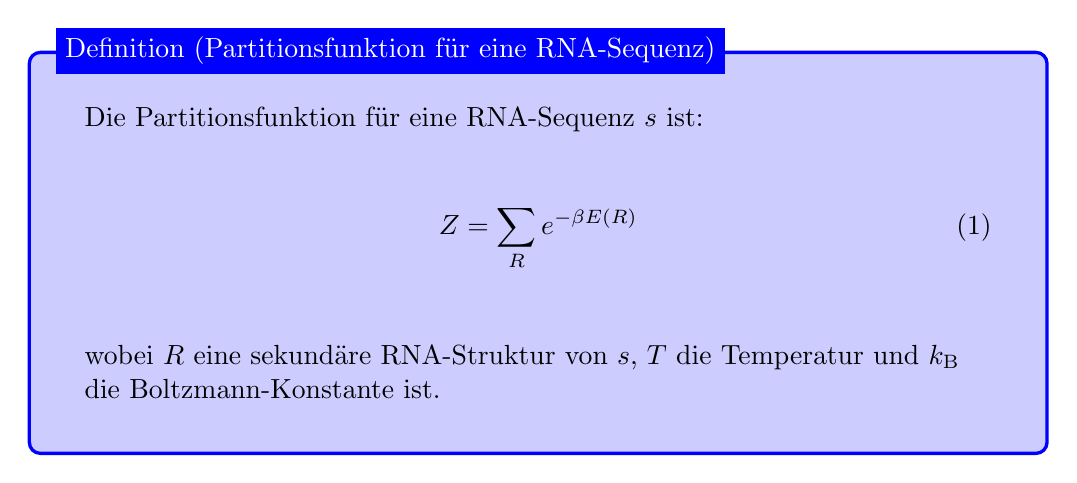
\begin{tikzpicture}
	\node [mybox] (box){%
    	Die Partitionsfunktion für eine RNA-Sequenz $s$ ist:
    	    	
		\vspace{1.5em}		
			\begin{equation}
				Z = \sum \limits_{R} e^{-\beta E(R)}
			\end{equation}					
		\vspace{1.5em}
		    	
    	wobei $R$ eine sekundäre RNA-Struktur von $s$, $T$ die Temperatur und $k_{\mathrm{B}}$ die Boltzmann-Konstante ist. 
	};
	\node[fancytitle, right=10pt] at (box.north west) {Definition (Partitionsfunktion für eine RNA-Sequenz)};
\end{tikzpicture}%  

\vspace{1.5em}

Der Algorithmus von McCaskill berechnet die Partitionsfunktion $Z$ für eine RNA-Sequenz $s$ effizient. Als Energiemodell für sekundäre RNA-Strukturen wird das Modell von Zuker benutzt. Das bedeutet, dass die Energie einer sekundären RNA-Struktur der Summe aller möglichen sekundären RNA-Strukturelemente entspricht.